\scanpage{10}
$k$ anneau commutatif
\[
S_n=k[[t_1,\ldots,t_n]]\qquad(n\ge0)
\]
\[
X_n=\operatorname{Spf}(S_n)
\]
$X_*=(X_n)_{n\ge0}$ schéma formel simplicial augmenté

$S_*=(S_n)_{n\ge0}$ anneau top. cosimplicial coaugmenté

On suppose donné, pour tout $n$\inserted{$\ge0$}, un sous-ensemble $\mathcal A_n\subset S_n$

On pose $\mathcal A_*=(\mathcal A_n)_{n\ge0}$. Un morphisme $X_m\xrightarrow{p}X_n$, associé à un hom de $k$-algèbres topologiques $S_n\xrightarrow{p^*}S_m$, est dit un \uline{$\mathcal A_*$-morphisme} si $p^*(t_i)=f_i\in S_m$ est $\in\mathcal A_m$ pour tout $1\le i\le n$.
\margin{\uline{NB} les $f_i$ sont tels que $\varepsilon(f_i)$ nilpotent}
\inserted{Donc ceci signifie que les $\operatorname{pr}_i\circ p$ $(1\le i\le n)$ sont des $\mathcal A_*$-morph.}
On suppose:

(a) Les opérations simpliciales entre les $X_n$ sont des $\mathcal A_*$-morphismes ($\Longleftrightarrow$ $\forall n\ge0$ et $1\le i\le n$ on a $t_i\in\mathcal A_n$; $\Longleftrightarrow$ les morphismes identiques des $X_n$ sont $\in\unsure{\mathcal A_n|\mathcal A_*}$)
\margin{Identités}

(b) Le composé de deux $\mathcal A_*$-morphismes est \unsure{Itou|un}
\margin{Composition}
[$\Longleftrightarrow$ si $p:X_m\longrightarrow X_n$ est un $\mathcal A_*$-morphisme, alors $p^*(\mathcal A_n)\subset\mathcal A_m$ $\Longleftrightarrow$ si $f_1,\ldots,f_n\in\mathcal A_m$, et $\varepsilon(f_1),\ldots,\varepsilon(f_n)$ nilpotents, alors pour tout $\varphi\in\mathcal A_n$\inserted{avec $\varepsilon(\varphi)$ nilpotent}, on a $\varphi(f_1,\ldots,f_n)\in\mathcal A_m$]
\margin{NB \deleted{\unsure{Ceci devient vrai}}\unsure{moyennant c)}, vrai (sans supposer $\varepsilon(\varphi)$ nilpotent donc \unsure{$=$} si $a\in\mathcal A_0$, \unsure{du fait que} $\operatorname{Im}(\mathcal A_0\to S_n)\subset\mathcal A_n$)}
\figure{\begin{tikzpicture}[x=1cm,y=1cm]\draw(0,1.5)..controls(.5,1.8)and(.5,1.2)..(.8,1.2);\draw(.8,1.2)..controls(.6,.5)and(.7,0)..(0,-.4);\end{tikzpicture}}
\deleted{
(c) Le morphisme ``différence'' $X_2=X_1\mathbin{\widehat\times}_kX_1\longrightarrow X_1$ $((x,y)\mapsto x-y)$ et ``produit'' $[(x,y)\mapsto xy]$ sont des $\mathcal A_*$-morphismes [$\Longleftrightarrow t_1-t_2$ et $t_1t_2$ sont $\in\mathcal A_2$,\inserted{et $1\in\mathcal A_0$} $\Longleftrightarrow$ les $\mathcal A_n$ sont \deleted{stables par des additions et produits, \unsure{et par des différences}} \unsure{des sous-groupes abéliens stables par produit}] \unsure{$\mathcal A$}
\deleted{\unsure{$1\in S_0$}}
}
\inserted{[sous-anneaux unitaires des $S_n$]}
\margin{condition annulaire}
\figure{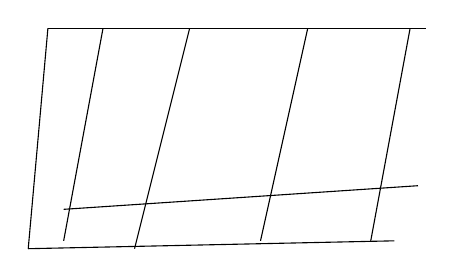
\begin{tikzpicture}[x=1cm,y=1cm]\draw(0,2.8)--(4.8,2.8);\draw(0,2.8)--(-.25,0);\draw(.7,2.8)--(.2,.1);\draw(1.8,2.8)--(1.1,0);\draw(3.3,2.8)--(2.7,.1);\draw(4.6,2.8)--(4.1,.1);\draw(-.25,0)--(4.4,.1);\draw(.2,.5)--(4.7,.8);\end{tikzpicture}}
\margin{9}
